\item[(f)]
\section{Impulse Response}

\subsection*{Problem Statement}
Plot the impulse response of the filter for \(0 \leq n \leq 50\).

\subsection*{Theoretical Background}
The impulse response of a digital filter is the output when the input is an impulse signal (a signal with a value of 1 at \( n = 0 \) and 0 elsewhere). The impulse response characterizes the filter completely in the time domain.

\subsection*{Implementation and Results}
The impulse response of the filter is computed and plotted using Python. The plot below illustrates the impulse response of the filter for \(0 \leq n \leq 50\).

\begin{figure}[h]
    \centering
    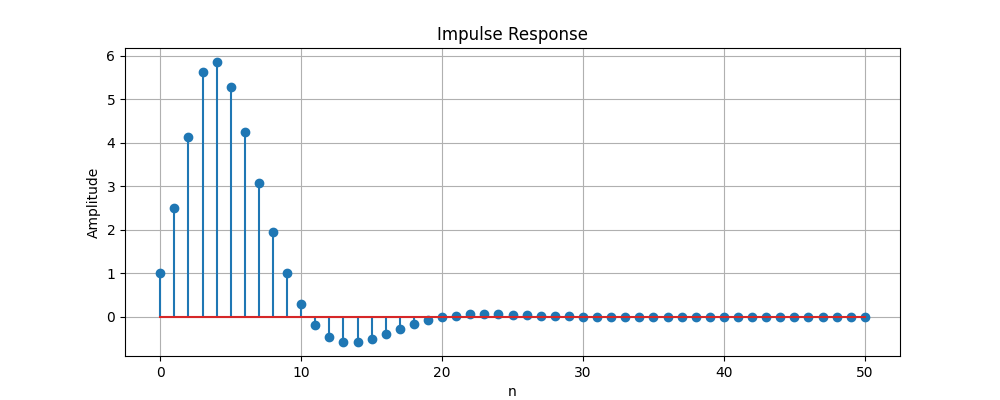
\includegraphics[width=0.8\textwidth]{fig/ex3_f_impulse_response.png}
    \caption{Impulse Response of the Filter}
    \label{fig:ex3_f_impulse_response}
\end{figure}

\subsection*{Conclusion}
The impulse response plot provides insights into the time-domain characteristics of the filter. It shows how the filter responds to an impulse input over time.
